\documentclass[a4paper,11pt]{beamer}
%	\documentclass[a4paper,11pt,handout]{beamer}

%%%%%%%%%%%%%%%%%%%%%%%%%%%%%%%%%%%%%%%%%%%%%%%%%%%%%%
%%%%%      Les packages de base                %%%%%%%
%%%%%%%%%%%%%%%%%%%%%%%%%%%%%%%%%%%%%%%%%%%%%%%%%%%%%%

\usepackage[utf8]{inputenc}  % pour taper directement les accents
\usepackage[T1]{fontenc}     % pour inclure les polices avec accents et gérer la césure des mots
\usepackage[french]{babel}	 % pour utiliser les règles de la typographie française
\usepackage{mathtools,amssymb,amsfonts}	% plus de math :-)
\usepackage{graphicx}	% c'est pour \includegraphics et \graphicspath
\usepackage{lastpage}   % \cfoot{\thepage $/$ \pageref{LastPage}}
\usepackage{ifthen}     % pour \ifthenelse
\usepackage{derivative}

\usepackage[locale = FR]{siunitx} % les unités PROPRES
\sisetup{inter-unit-product = \ensuremath{{}\cdot{}}}

\usepackage{pgfplots}  % environnement axis
\pgfplotsset{compat=1.15}

\usepackage{tikz}
\usetikzlibrary{calc}  % pour faire des calculs sur les coordonnées ($(A)+(45:3)$)

\usepackage{tikzelec}  % package maison pour dessiner les circuits électroniques

%%%%%%%%%%%%%%%%%%%%%%%%%%%%%%%%%%%%%%%%%%%%%%%%%%%%%%
%%%%%  Pour numeroter les pages                %%%%%%%
%%%%%%%%%%%%%%%%%%%%%%%%%%%%%%%%%%%%%%%%%%%%%%%%%%%%%%

\setbeamertemplate{navigation symbols}{}
%=======================================================
% Pour numéroter les diapos :
\setbeamertemplate{footline}[frame number]
%=======================================================
% Pour numéroter les diapos en choissant le numéro de la dernière
% dans ce cas enlever la commande \setbeamertemplate{footline}[page number]
% et utiliser les deux lignes suivantes
\newcommand {\NumeroDerniereDiapo} {22}
%\addtobeamertemplate{footline}{\hfill\insertframenumber\,/\,\NumeroDerniereDiapo\hspace{2mm}\null\vspace{1mm}}
%=======================================================

%%%%%%%%%%%%%%%%%%%%%%%%%%%%%%%%%%%%%%%%%%%%%%%%%%%%%%
%%%%%  Pour positionner les choses où on veut  %%%%%%%
%%%%%%%%%%%%%%%%%%%%%%%%%%%%%%%%%%%%%%%%%%%%%%%%%%%%%%

\usepackage[absolute,showboxes,overlay]{textpos}
\textblockorigin{10mm}{10mm} % origine des positions
\setlength{\TPHorizModule}{1mm} % échelle horizontale
\setlength{\TPVertModule}{\TPHorizModule} % échelle verticale identique à l'horizontale

% à ajouter dans les frames pour positioner les objets
% \begin{textblock}{largeur}(x,y) (les nombres sont en mm) :
%
%%\TPshowboxestrue  % (par défaut) les boites sont visibles
%%\TPshowboxesfalse % décommenter pour faire disparaitre les boites
%
%\begin{textblock}{115}(-3,10)
%bla bla
%\end{textblock}
%


\newenvironment{tikzgrille}[1][0]{
% 1 pour afficher la grille / 0 pour ne pas l'afficher = option par défaut
\begin{textblock}{180}[.5,.5](54,38)
\begin{tikzpicture}
\draw (-9,-9) rectangle (9,9);
\ifthenelse {#1=1} {\begin{scope}[magenta!60]
\draw (-9,-9) grid (9,9);
\fill (0,0) circle (.05);
\fill (1,0) circle (.05);
\fill (0,1) circle (.05);
\node[anchor=text] at (0.1,0.2) {\footnotesize $(0,0)$};
\node[anchor=text] at (1.1,0.2) {\footnotesize $(1,0)$};
\node[anchor=text] at (0.1,1.2) {\footnotesize $(0,1)$};
\end{scope}} {} }
{\end{tikzpicture}\end{textblock}}

\newcommand{\eff}{_\text{eff}}
\newcommand{\cel}{\degreeCelsius}

%%%%%%%%%%%%%%%%%%%%%%%%%%%%%%%%%%%%%%%%%%%%%%%%%%%%%%
%%%%%%%%%%%%%%%%%%%%%%%%%%%%%%%%%%%%%%%%%%%%%%%%%%%%%%

\title{Consommation électrique d'un data-center}
\author{Malo Leroy, Ulysse Tanguy-Bompard}

\begin{document}

%=====================================================
%=====================================================
%=====================================================

\maketitle % diapo-titre


\begin{frame}
\frametitle{Ancrage au thème et motivation}
Ancrage : augmentation de l'usage des technologies numériques

Motivation : écologie, enjeux économiques
\end{frame}

\begin{frame}
    \frametitle{Plan}
    \begin{enumerate}
        \item Modélisation par un circuit équivalent
        \item Influence de la quantité de calculs
        \item Influence de la température
        \item Objectifs futurs
    \end{enumerate}
\end{frame}

\begin{frame}
    \frametitle{Modélisation}
    \framesubtitle{par des circuits éléctriques simples}

    $$U\eff = \SI{230}{V} \quad I\eff = \SI{0,20}{A} \quad \text{et} \quad \cos \varphi = \SI{0,7}{}$$

    \begin{columns}
        \def \x {0} % origine
        \def \xa {2}
        \def \xb {4.5}
        \def \xc {6}

        \def \y {0} % origine
    \begin{column}{0.33\textwidth}
    \begin{tikzelec}
        \draw (\x, \y)--(\xc, \y);

        \TikzelecResistance \xa \y
        \TikzelecNom {$R$}    {0}   {1}

        \TikzelecCondensateur \xb \y
        \TikzelecNom {$C$}    {0}   {1}

        \node at (\xa, -3) {$R = \SI{1,6}{k\ohm}$};
        \node at (\xa, -4.2) {$C = \SI{1,9}{\micro F}$};
    \end{tikzelec}
    \end{column}
    \begin{column}{0.33\textwidth}
    \begin{tikzelec}
        \draw (\x, \y)--(\xc, \y);

        \TikzelecResistance \xa \y
        \TikzelecNom {$R$}    {0}   {1}

        \TikzelecBobine \xb \y
        \TikzelecNom {$L$}    {0}   {1}

        \node at (\xa, -3) {$R = \SI{800}{\ohm}$};
        \node at (\xa, -4.2) {$L = \SI{2,6}{H}$};
    \end{tikzelec}
    \end{column}
    \begin{column}{0.33\textwidth}
        \def \xe {3}
        \def \xf {4}
        \def \yd {-2}
        \begin{tikzelec}
            \draw (\x, \y)--(\xf+1, \y);
            \draw (\xa-1, \y)--(\xa-1, \yd);
            \draw (\xa-1, \yd)--(\xf, \yd);
            \draw (\xf, \yd)--(\xf, \y);

            \TikzelecCondensateur {\xa+.5} \y
            \TikzelecNom {$C$}    {0}   {1}

            \TikzelecResistance {\xa+.5} \yd
            \TikzelecNom {$R$}    {0}   {-1}

            \node at (\xa, -4.5) {$R = \SI{1,6}{k\ohm}$};
            \node at (\xa, -5.8) {$C = \SI{2,0}{\micro F}$};
        \end{tikzelec}
    \end{column}
    \end{columns}
\end{frame} % modélisation

\begin{frame}
    \frametitle{Influence de la quantité de calculs}

    \begin{enumerate}
        \item Étude qualitative : $\pdv{I\eff}{K} > 0$ ($K \nearrow ~\Rightarrow~ I\eff \nearrow$)
        \item Étude quantitative
    \end{enumerate}

    \begin{tikzpicture}
        \node at (2, 0) {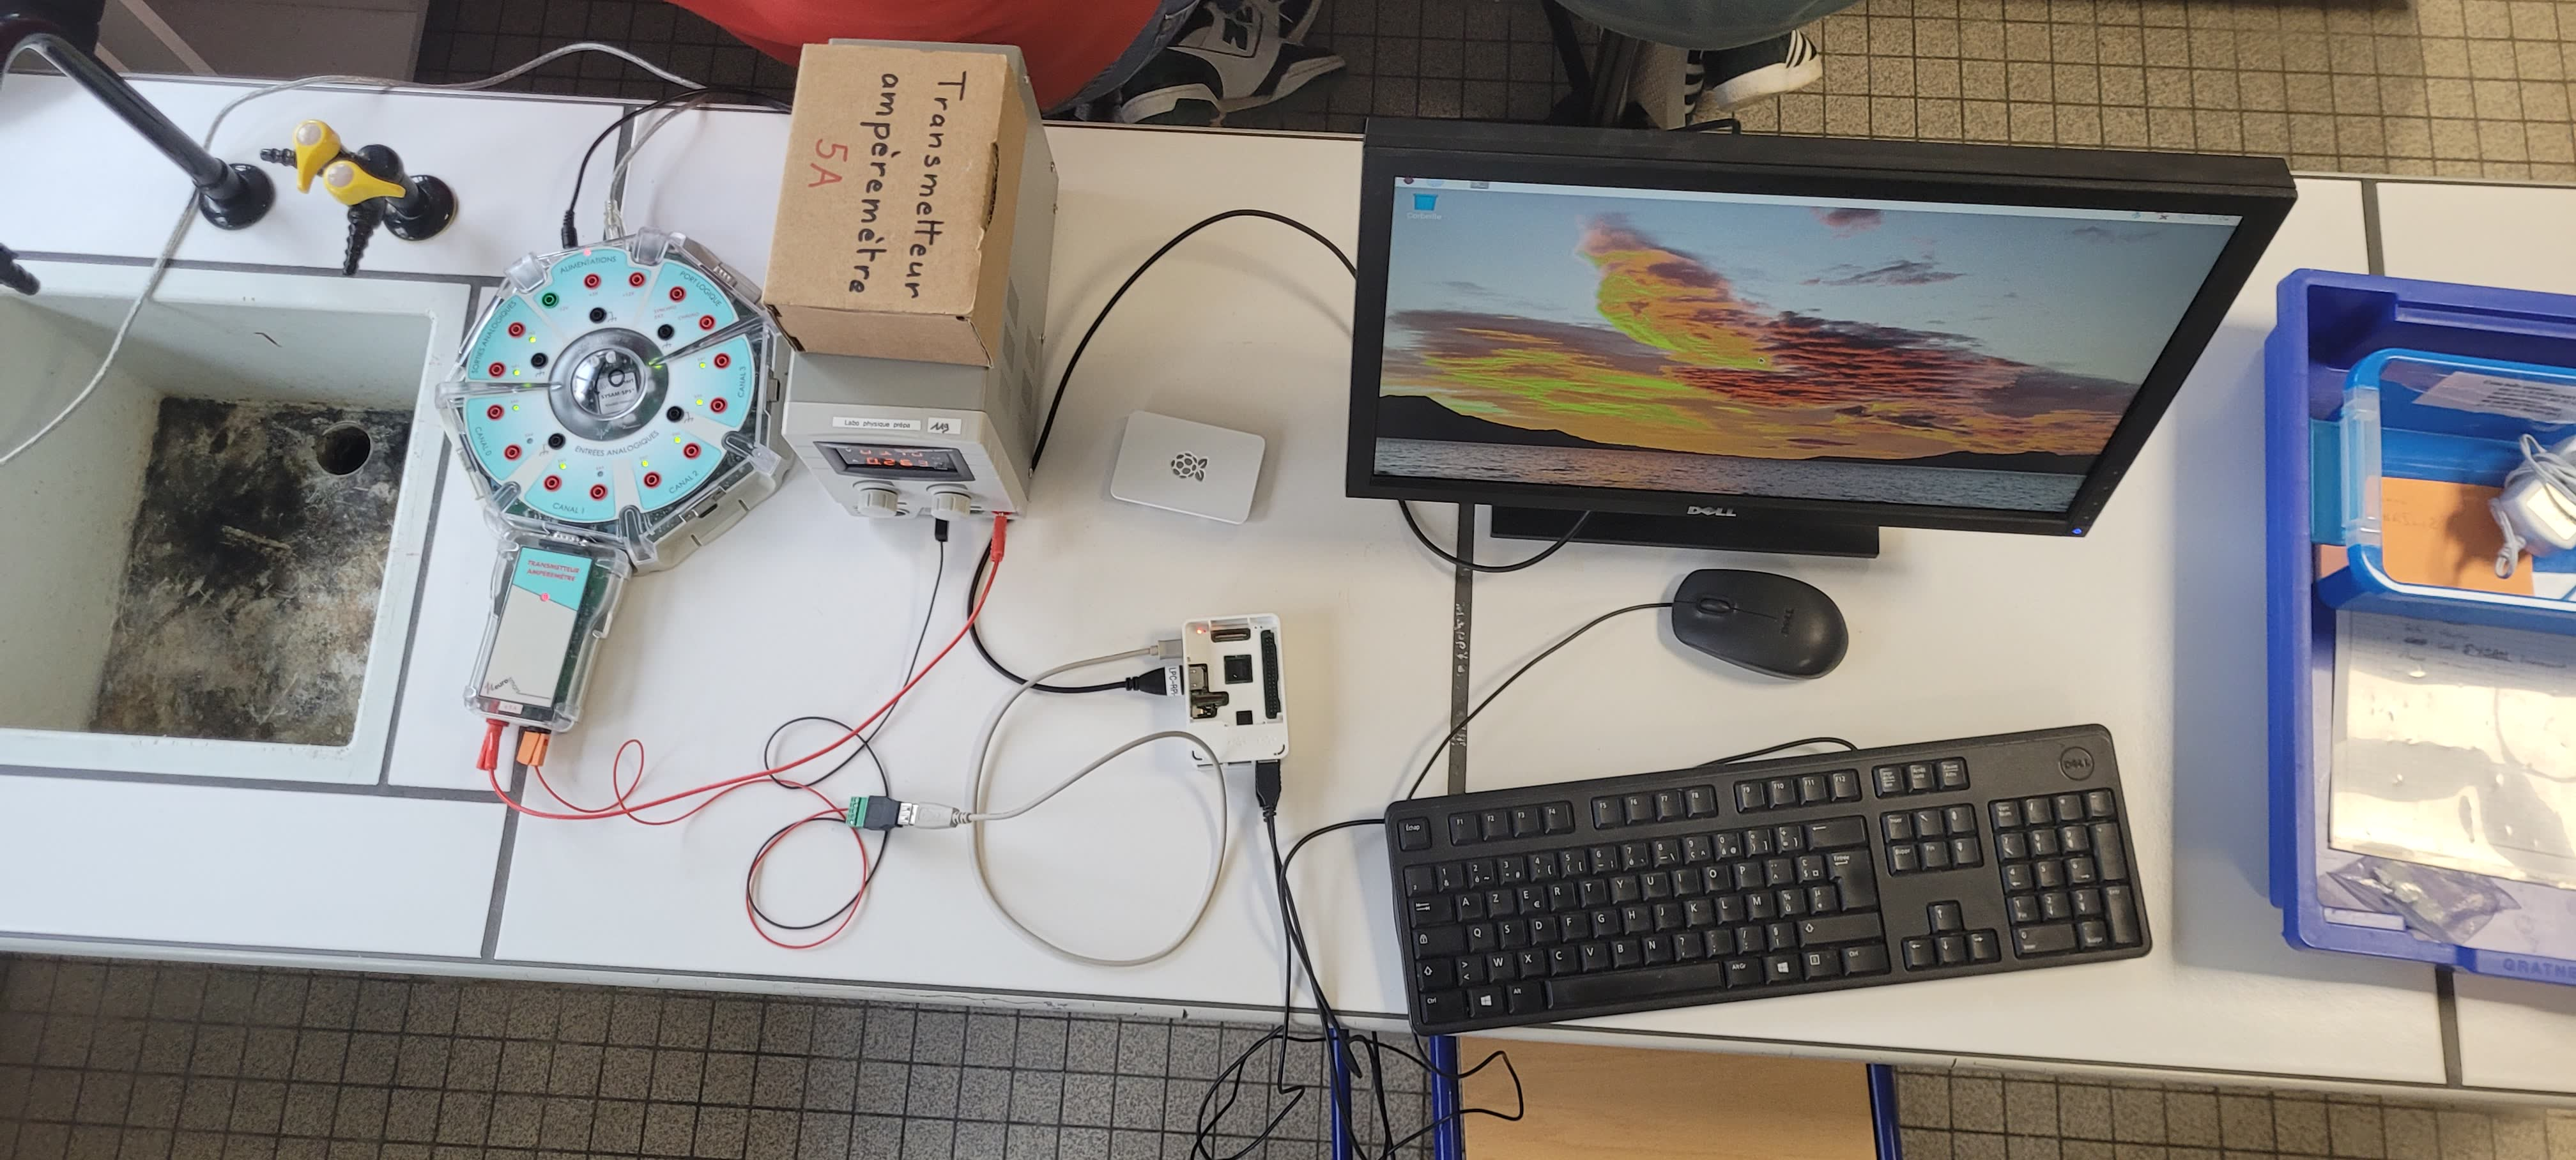
\includegraphics[width=0.8\textwidth]{../images/TP-2.1.jpg}};
        \node at (-1, -3) {Carte Sysam};
        \node at (2, -3) {Raspberry Pi};

        \draw[red, ->] (-1, -2.5) -- (-0.5, 0);
        \draw[red, ->] (2, -2.5) -- (1.8, -0.5);
    \end{tikzpicture}

\end{frame} % calculs: tp

\begin{frame}
    \frametitle{Influence de la quantité de calculs}

    \begin{tikzpicture}
    \begin{axis}[
        width = 10cm, height = 6cm,
        domain=0:4000,
        title  = {Intensité en fonction de la quantité de calculs},
        xlabel = {$K$ (calculs par seconde)},
        ylabel = {$I\eff(K)$ (mA)},
        grid,
        xtick = {0,1000,...,4000},
        legend pos = north west,
    ]

    \addplot [blue, only marks] coordinates {
    (0, 200)
    (100, 230)
    (1000, 360)
    (3900, 600)
    };
    \end{axis}

    \node at (4,-1.8) {Avec plus de points on pourra proposer un modèle};
    \end{tikzpicture}
\end{frame} % calculs

\begin{frame}
    \frametitle{Influence de la température}

    \begin{enumerate}
        \item Étude qualitative $\pdv{I\eff}{T} > 0$ ($T \nearrow ~\Rightarrow~ I\eff \nearrow$)
        \item Étude quantitative
        \begin{center}
            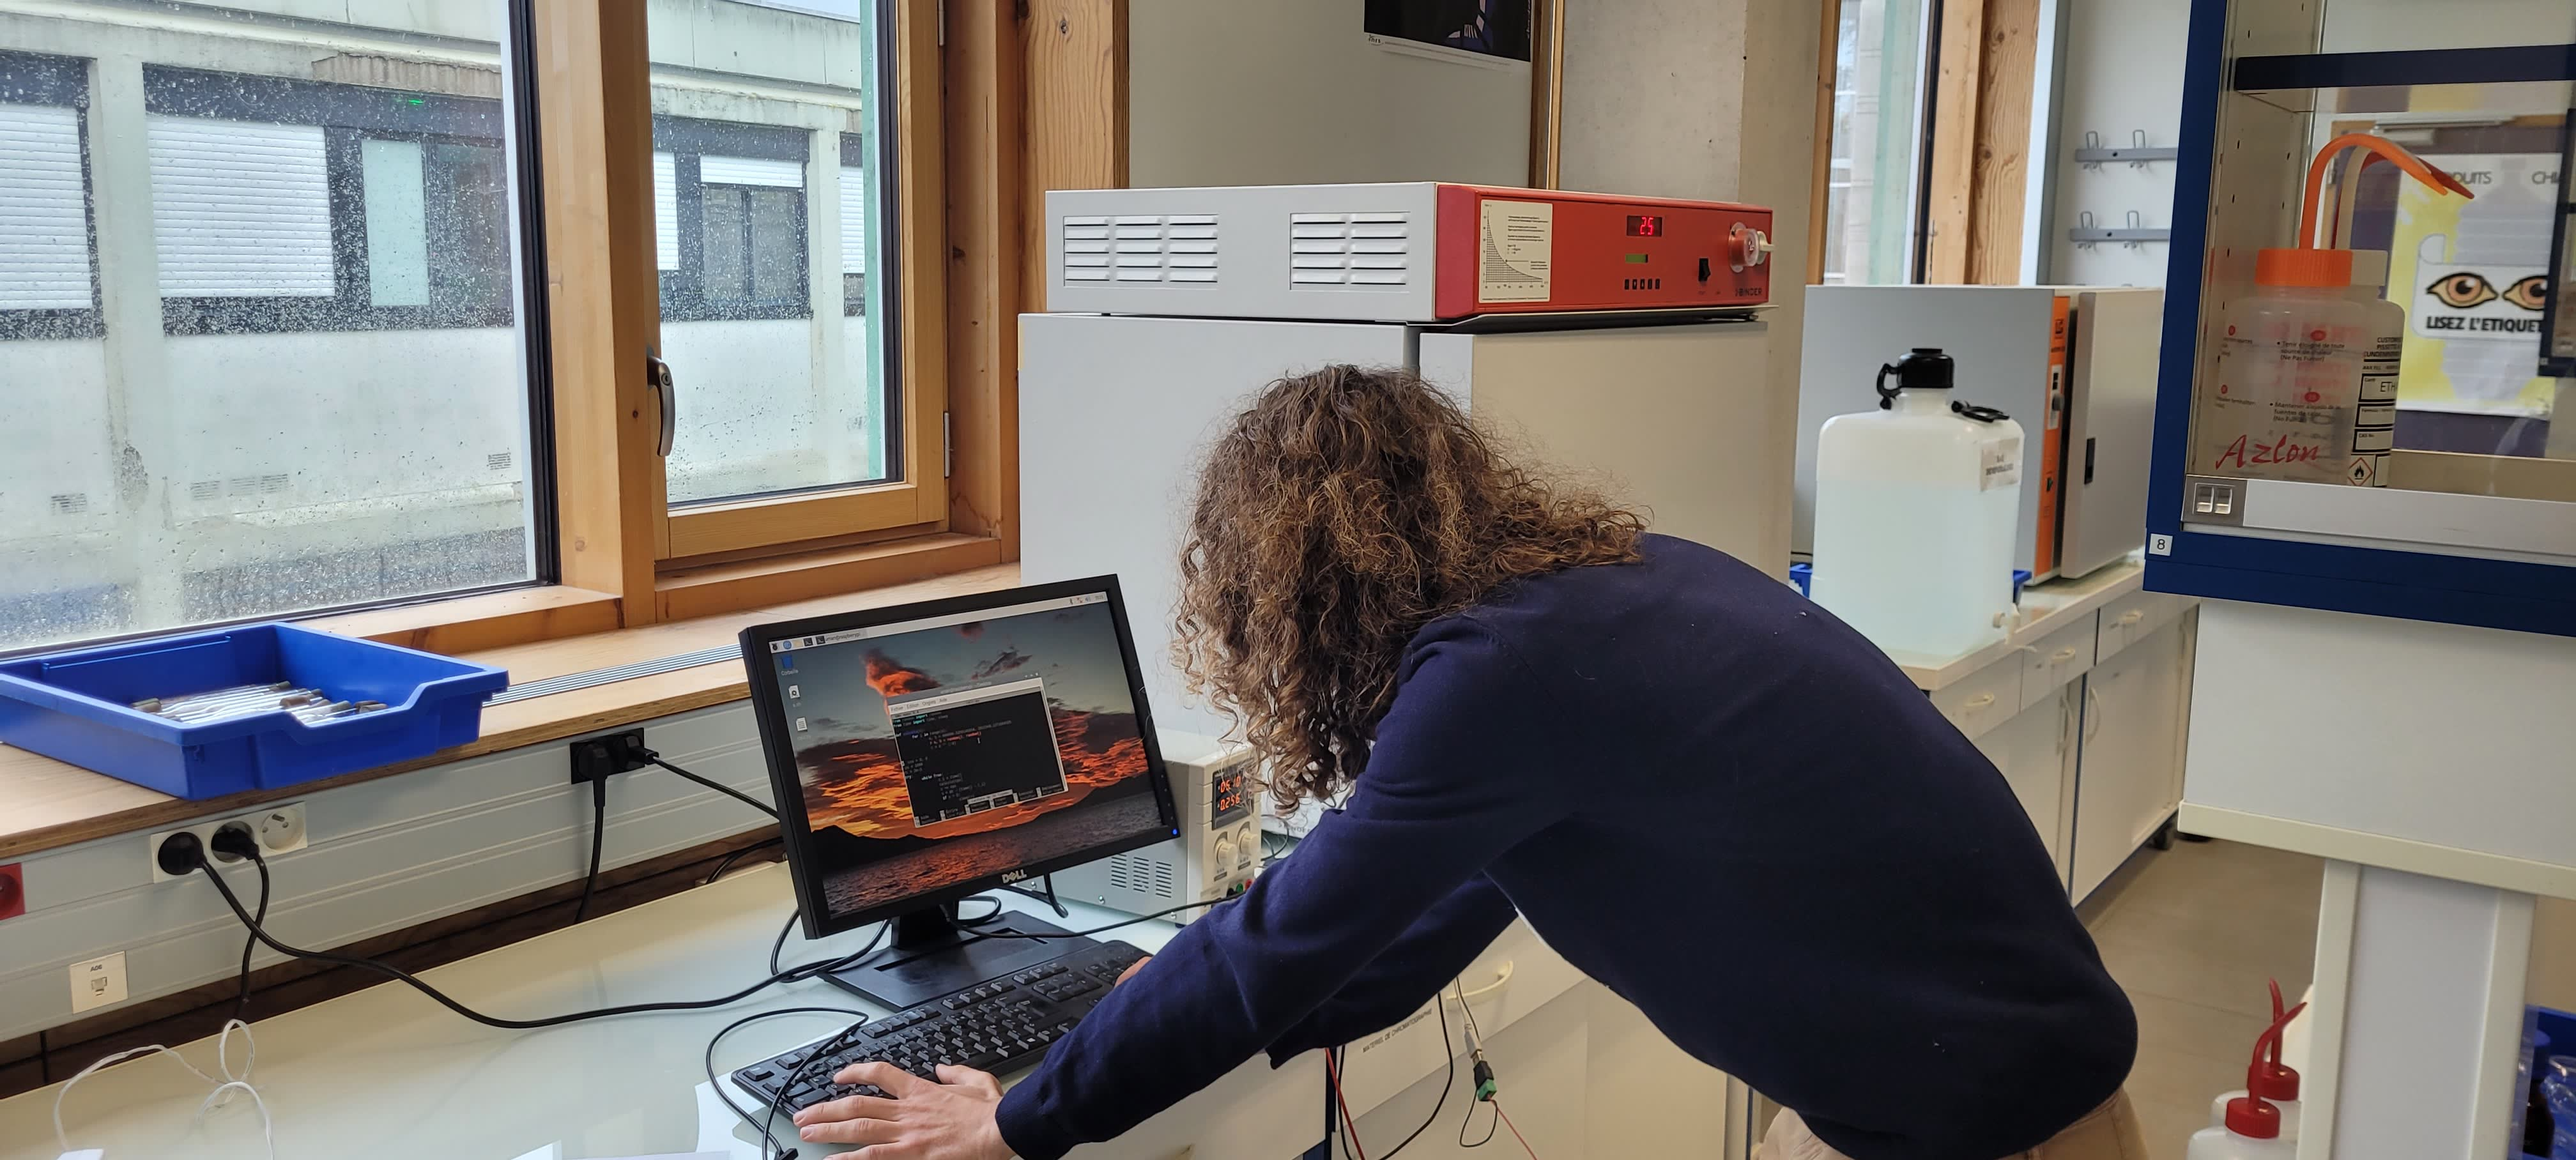
\includegraphics[width=0.8\textwidth]{../images/TP-2.3.jpg}
        \end{center}
    \end{enumerate}
\end{frame} % température: tp

\begin{frame}
    \frametitle{Influence de la température}

    \begin{tikzpicture}
    \begin{axis}[
        width = 10cm, height = 6cm,
        domain=0:60,
        title  = {Intensité en fonction de la température extérieure},
        xlabel = {$T$ (en \SI{}{\cel})},
        ylabel = {$I\eff(K)$ (mA)},
        grid,
        xtick = {20,25,...,60},
        legend pos = south east,
    ]

    \addplot [blue, only marks] coordinates {
        (31, 268)
        (35, 268)
        (41, 267)
        (46, 274)
    };

    \addplot [red, only marks] coordinates {
        (31, 304)
        (35, 310)
        (46, 310)
        (56, 310)
    };

    \legend{$K = 0$, $K = 1000~\text{cps}$}

    \end{axis}

    \node at (4,-1.8) {Problème : temps de thermalisation};

    \end{tikzpicture}
\end{frame} % température

\begin{frame}
    \frametitle{Objectifs futurs}

    Ce qui a été fait :
    \begin{itemize}
        \item $I = f(K, T)$ (en cours)
    \end{itemize}

    Ce qui reste à faire :
    \begin{itemize}
        \item Détermination de $C_{eq}$, $\lambda_{eq}$ et $h$ (coef. de Newton)
        \item Divers modèles d'interaction thermique % entre plusieurs ordinateurs
        \item Optimisation de la répartition des calculs
    \end{itemize}
\end{frame}

%=====================================================
%=====================================================
%=====================================================

\end{document}
